\documentclass[a4paper,12pt,oneside]{scrreprt}
\usepackage[latin1]{inputenc}
\usepackage[T1]{fontenc}
\usepackage{ae,aecompl}
\usepackage[english]{babel}
\usepackage{amsmath}
\usepackage{amssymb}
\usepackage{amsfonts}
\usepackage{amsthm}
\usepackage{graphicx}
\usepackage{wrapfig}
\usepackage{ulem}
\usepackage{cancel}
\usepackage{float}
\usepackage{color}
%\usepackage{titlesec}
\usepackage{geometry}
\geometry{verbose,a4paper,tmargin=25mm,bmargin=25mm,lmargin=15mm,rmargin=25mm}
%\titlelabel{\thetitle.\quad}
\usepackage{tabularx}
\usepackage{booktabs}
\usepackage{paralist}
\usepackage{textcomp}
\usepackage[official]{eurosym}

\renewcommand{\rmdefault}{phv}
\renewcommand{\sfdefault}{phv}

% for splitting page into many pages vertically
\usepackage{paracol}

% our OWN imports for our use
\usepackage{listings}
\lstdefinestyle{ourJavaStyle}{
	language=Java,
	%numbers=left,
	%numbersep=8pt,
	stepnumber=1,
	tabsize=2,
	showspaces=false,
	showstringspaces=false,
	basicstyle=\ttfamily\scriptsize,
	keywordstyle=\color{blue}\ttfamily,
	stringstyle=\color{red}\ttfamily,
	commentstyle=\color{green}\ttfamily,
	breaklines=true
}

\newcommand*{\sourcepath}{../code/src/main/java}
\newcommand*{\testpath}{../code/src/test/java}

\renewcommand{\thesubsection}{\thesection.\alph{subsection}}
%\titleformat{\subsection}
%{\normalfont\fontfamily{phv}\fontsize{14}{17}\bfseries}{\thesubsection}{1em}{}

\begin{document}
	
	\begin{tabular}{ccc}
		\begin{large} \textbf{Prof. Lichter} \end{large} &
		
		\begin{minipage}[H]{3.5cm}
			\centering
			\begin{large} OOSC \end{large} \\
			\begin{large} WS 2019/2020 \end{large}
		\end{minipage} &
		
		\begin{minipage}[H]{4cm}
			
\includegraphics[keepaspectratio,width=\textwidth,angle=0]{images/swc.png}
		\end{minipage} \\
		Andreas Steffens, Konrad F\"ogen &  &  \\
		& \begin{huge} \textbf{Submission 2} \end{huge}&  \\
		& oosc@swc.rwth-aachen.de &  \\
		& & \\
		% Hier drunter muessen die Daten noch angepasst werden
		Issued: 04.11.2019 &
		Submission: 18.11.2019 &
		Discussion: 21.11.2019 \\
	\end{tabular}
	\newline \newline \newline
	\centering
	Submitted by Group 10
	
	\begin{tabular}{ll}
		Dominik Bittner, & 369202 \\
		Ulfet Cetin, & 391819\\
		Philipp Hochmann, & 356148 \\
		Anar Orujov, & 391825\\
		Ada Slupczynski, & 384147\\
		(sorted on lastname basis)
	\end{tabular}
    
	\setcounter{chapter}{2} % Aktuelles Assigment
	\section{Assignment:}
	
    % TODO: Image of the UML is missing
    
	\begin{table}[h]
		\centering
		\resizebox{\textwidth}{!}
		{%
			\begin{tabular}{|l|l|}
				\hline
				\multicolumn{1}{|c|}{\textbf{Statement}} & \multicolumn{1}{c|}{\textbf{Output or Description of Failure}} \\ \hline
				cow.writeName();                         & output: "Cow"         \\ \hline
				aurochs.writeName();                     & output: "Aurochs"     \\ \hline
				((Material)aurochs).writeName();         & output: "Material"    \\ \hline
				((Aurochs)cow).writeName();              & output: "Aurochs"     \\ \hline
				((Cow)aurochs).writeName();              & output: 
                "Cow"         \\ \hline
				aurochs.writeLatin();                    & output: "Bos primigenius"  \\ \hline
				auerochse.writeDescription();              & fail:
                variable auerochse is not defined.      \\ \hline
				((Aurochs)material).writeName();         & fail: we cannot limit to subclass, variable material is not a Aurochs.
				                                                                 \\ \hline
			\end{tabular}
		}
	\end{table}
	
	\section{Assignment:}
    
    In the given class diagram inheritance is not implemented as a "is a"-relation. 
    
    \begin{enumerate}
        \item A cover is not a book, so it sould not inherite from it.
        \item There is something mixed up with literature and text as content:
        \begin{itemize}
            \item Literature is not necessary a single text. It may contains of more than one.
            \item A book is literature, but includes much text.
        \end{itemize}
        \item A paper is not a book.
    \end{enumerate}

    Most of the associations are correct. But the associations from the author may be reversed. Instead giving the author a list of written text -- and additionally a list of written papers -- you can give each text an author.
    
    This leads to the conclusion, that the quality how inheritance and
    association was implemented here, is not very good nor consistent.
    
    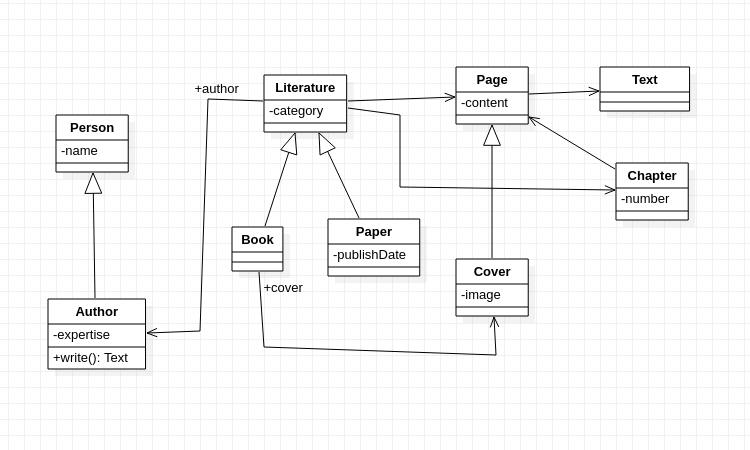
\includegraphics[width=\textwidth]{../uml/2_2.png}
    
    In this class diagram the \textit{Text}-class is separated. Instead \textit{Literature} is the parent of \textit{Book} and \textit{Paper}. So a paper is no longer a book. Each literature has an author. The author is still a person, but now can write texts by itself. Some texts are summarized in a \textit{Page}. A \textit{Cover} is a special kind of page with an image. \textit{Chapter}s bind some pages together. But a \textit{Literature} still have a list of pages and a list of chapters separatly.
    
	\section{Assignment:}
    
    \begin{flushleft}
        This inheritance hierarchy fits in two types of Meyer's inheritance taxonomy:
        \begin{enumerate}
            \item Subtype Inheritance: The Circle and the Ellipse are both GeoObjects. So there is a 'is-a' relation between GeoObject and it's subclasses.
            \item Extension Inheritance: Both child classes provides new functionallity which doesn't fit to a GeoObject. Not every GeoObject has a diameter.
        \end{enumerate}
    
        In the code there is no redefinition, so it doesn't fit into Variation Inheritance nor Uneffective Inheritance. Also the \textit{GeoObject} is not abstract, so it doesn't fit into the Reification Inheritance nor the Structure Inheritance. As well it doesn't fit into Implementation Inheritance, because the child objects don't make use of any functionallity which is provided by the parent.
        
        % TODO: View, Restriction and Facility
        
        But in both cases there is a point, that could be improved. If the author want to use a Subtype Inheritance, it would make sense to make \textit{Circle} a subclass of \textit{Ellipse}. Because every circle is a ellipse. Than it is not necessary to provide the same implementation for the diameter-methods again.
        
        If the author want to use a Extension Inheritance the hierarchy could be changed in that way, that \textit{Ellipse} is a subclass of \textit{Circle}. The ellipse provides more functionallity than the circle. So there is still an extension but the diameter-methods don't have to be implemented again.
    \end{flushleft}
	
	\clearpage
	\section{Assignment:}
		

\begin{figure}[H]
	\centering 
	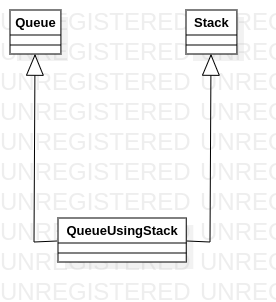
\includegraphics[clip, trim=0cm 0cm 0cm 0cm, scale=0.3]{q5/images/q5_classdiagram.png}
	\caption{Implementation Inheritance Diagram}
\end{figure}

\noindent\begin{minipage}{.45\textwidth}
	\lstinputlisting[style=ourJavaStyle, firstline=0,lastline=44]{\sourcepath /Q5/QueueUsingStack.java}
\end{minipage}\hfill
\begin{minipage}{.45\textwidth}
	\lstinputlisting[style=ourJavaStyle, firstline=45,lastline=90]{\sourcepath /Q5/QueueUsingStack.java}
\end{minipage}
\clearpage

\begin{itemize}
	\item This is implementation inheritance, because a queue class called QueueUsingStack is implemented using Stack class:
		\begin{compactitem}
			\item both QueueUsingStack and Stack classes are \textbf{concrete}\\
			(we implemented Stack ourselves)
			
			\bigskip
			
			\item QueueUsingStack obtains features that are NOT constant, those features are put to use for implementation of functionality of QueueUsingStack.\\
			(direct use of features of Stack to implement functionalities of QueueUsingStack)
		\end{compactitem}
	
	\item This is not some other inheritance of Meyer approach:
		\begin{compactitem}
			\item not a \textbf{reification inheritance}
				\begin{compactitem}
					\item none of the classes are abstract
					\item the idea that class A representing `general kind of data structure`, and B being partial or complete implementation of A DOES NOT hold. (Queue is not some type of stack)
				\end{compactitem}
				\bigskip
			
			\item not a \textbf{structure inheritance}
				\begin{compactitem}
					\item there is no inheritance in our design where a class named A represents a structural property (like `Serializable`), and some other class B inherits from class A.
				\end{compactitem}
				\bigskip
				
			\item not a \textbf{facility inheritance}
				\begin{compactitem}
					\item ours is not a `constant inheritance`, no class of ours that are inherited have constant features (for that matter, we have no constant features)
					\item ours is not a `machine inheritance`, no functionality on our inherited class that can be considered as `functions on abstract machine`.
				\end{compactitem}
		\end{compactitem}
		
		
	\item How to avoid implementation inheritance?
		\begin{compactitem}
			\item we could have applied structure inheritance (like the one given in the lecture slides). 
				\begin{compactitem}
					\item There should have been `UsingStack` class between the inheritance chain between QueueUsingStack and Stack.
					Instead of QueueUsingStack $\Rightarrow$ Stack, we could have had QueueUsingStack $\Rightarrow$ UsingStack (use)$\Rightarrow$ Stack
				\end{compactitem}
				\bigskip
				
			\item exploiting `use-relation`
				\begin{compactitem}
					\item we could have removed `extends Stack` part (together with the redefinition part)
					\item we could have imported two Stack objects (mainStack, helperStack) instead of one(helperStack), and instead of using `list` object that is inherited from Stack object, we could have used mainStack object
					\item doing these two prerequisites, we would have had use-relation, as we would only use instances of Stack, and we would not redefine and extend it.
					\bigskip
					
					\item Our example both uses Implementation Inheritance and use-relation. Nevertheless, there is an Implementation Inheritance in it. We could have get rid of use-relation in its original form, and could have used other data structure, but in order to explain the reconstruction using use-relation, we deemed this way to be a fit for the assignment.
				\end{compactitem}
		\end{compactitem}
	
	\item Respective JUnit tests could be found in the submission: \\
	at code/src/test/java/Q5/QueueUsingStackTest.java
		
\end{itemize}
	\section{Assignment:}
	\section{Assignment:}
	\section{}
	\newpage
\subsection{}

    Rough steps:
    \begin{enumerate}
        \item Read string from console
        \item Tokenize string (Read chars until operator is found, substrings between operators are constants or variables)
        \item Parse token-stream to operator tree (e.g. with Dijkstra's famous shunting yard algorithm)
        \item Optionally post process operator tree to simplify it
    \end{enumerate}

    \begin{figure}[H]
        \centering
        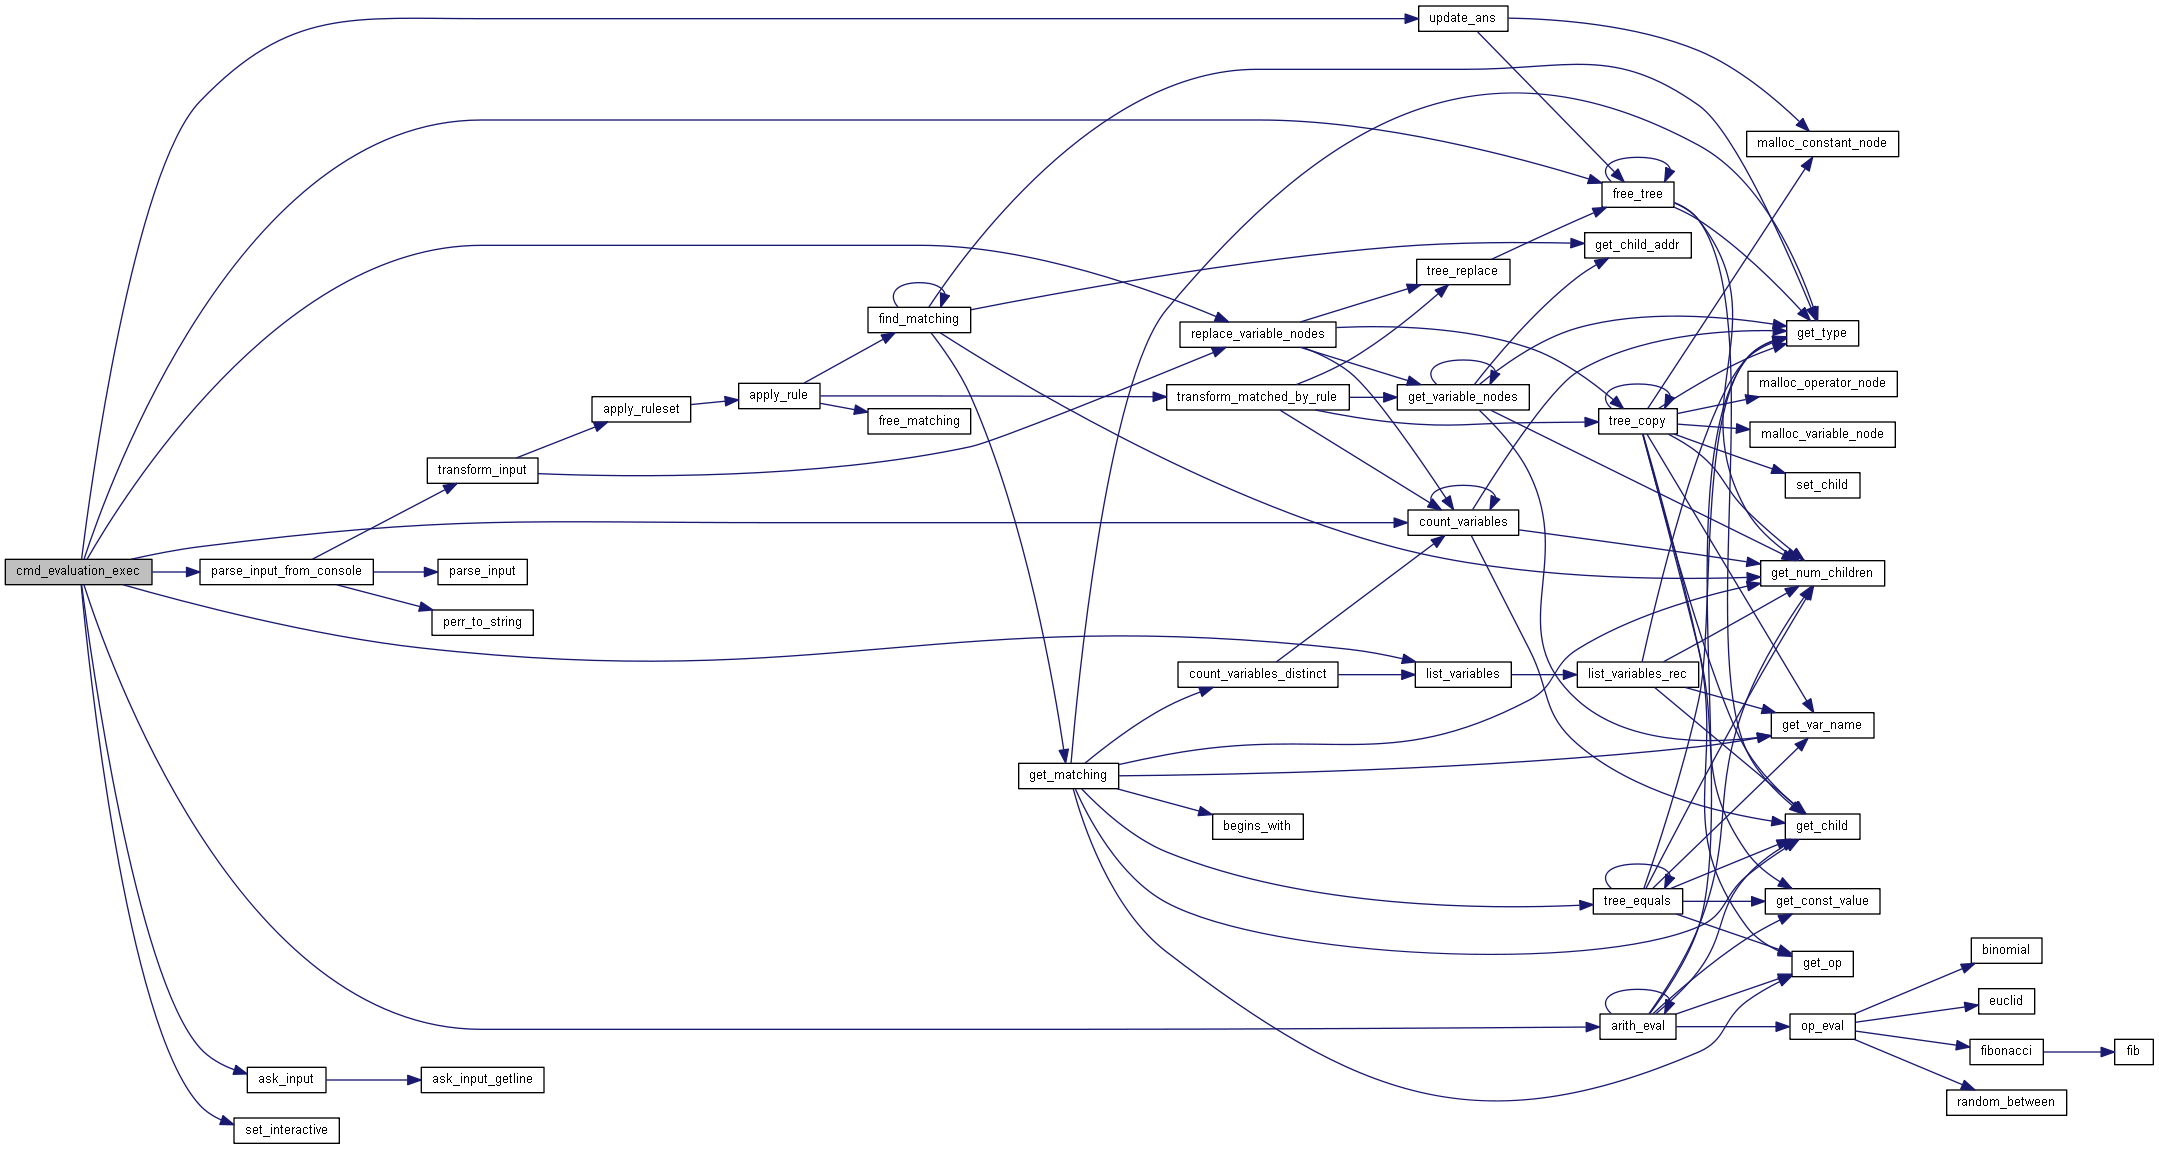
\includegraphics[width=\linewidth]{images/ex7/read_and_simplify.png}
        \caption{To read string from console and simplify it (step 1 and 4)}
    \end{figure}

    \begin{figure}[H]
        \centering
        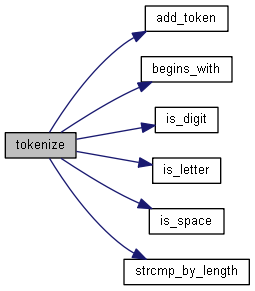
\includegraphics[width=0.3\linewidth]{images/ex7/tokenize.png}
        \caption{To tokenize it (step 2)}
    \end{figure}

    \begin{figure}[H]
        \centering
        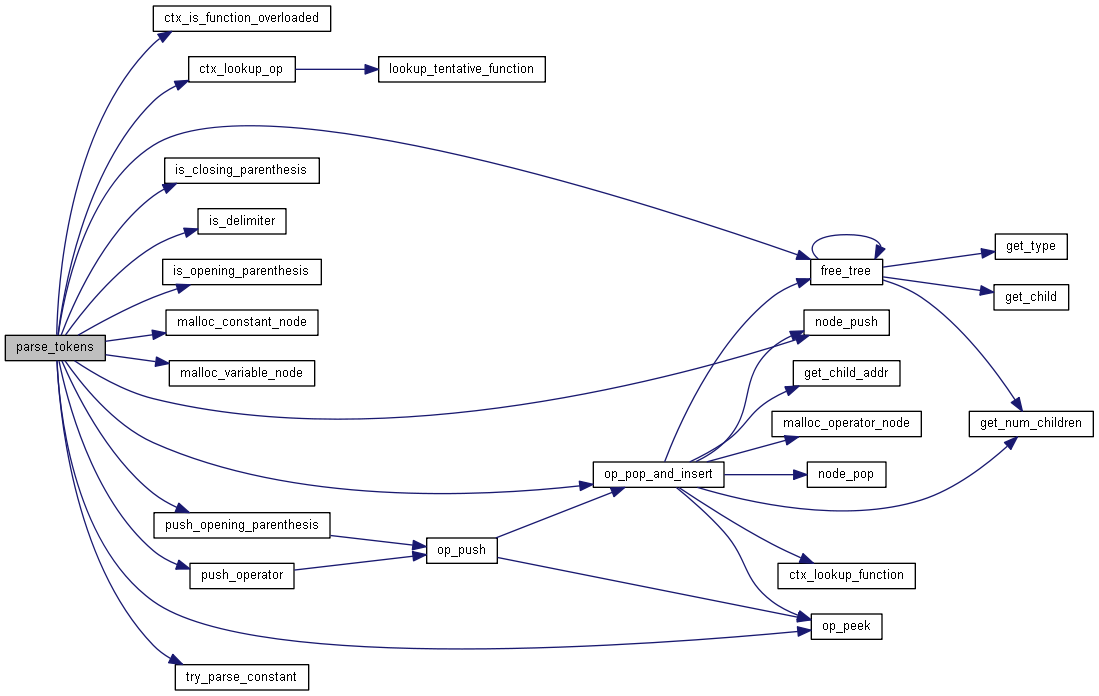
\includegraphics[width=\linewidth]{images/ex7/parse.png}
        \caption{To parse it (step 3)}
    \end{figure}

\subsection{2}
See given Java code

\subsection{3}
See given Java code
	\section{}
	\subsection{}

\begin{enumerate}
\item Factory Method: This pattern supports universal polymorphism, since it can return objects of potentially infinitely many derived types. It is a common pattern to avoid calling a constructor of a specific derived type directly. It is better to call a factory than to call a constructor, if the factory should decide which concrete subclass to use, or if additional subclasses may be added to the application in the future. In the example code given, a factory to construct a node from a token (see ex. 7) is given. The returned Node is polymorphic, because it may be an OperatorNode when the supplied token is a string that matches an operator, or a ConstantNode when the supplied token matches a number.
\item todo
\item todo
\end{enumerate}
\end{document}